

%%% This LaTeX source document can be used as the basis for your technical
%%% report. Intentionally stripped and simplified
%%% and commands should be adjusted for your particular paper - title, 
%%% author, citations, equations, etc.
% % Citations/references are in report.bib 

\documentclass[conference,backref=page]{acmsiggraph}
\usepackage{algorithm2e}
\usepackage{graphicx}
\usepackage{pgfplots}
\TOGonlineid{45678}
\TOGvolume{0}
\TOGnumber{0}
\TOGarticleDOI{1111111.2222222}
\TOGprojectURL{}
\TOGvideoURL{}
\TOGdataURL{}
\TOGcodeURL{}

% Include this so that citations show up in blue and the page information is included in the reference section
\hypersetup{
    colorlinks = true, 
    linkcolor = blue,
    anchorcolor = red,
    citecolor = blue, 
    filecolor = red, 
}

\title{Travelling Salesman Problem\\
	   Report}

\author{Conner Weatherston \thanks{e-mail:40167111@live.napier.ac.uk} \\
Edinburgh Napier University\\
Algorithms and Data Structures (SET09117)}
\pdfauthor{Conner Weatherston}

\keywords{travelling salesman problem, nearest neighbour, optimisation, algorithms}

\begin{document}

\maketitle

\raggedbottom

\begin{abstract}

The purpose of this report is to find out the efficiency of the nearest neighbour algorithm in order to solve a  variety of travelling salesman problems. This report is also looking how possible variations and optimization techniques such as just searching on an individual axis in order to improve upon the algorithm. ADD SENTENCE SUMMARY. 
\end{abstract}



\keywordlist


\section{Introduction}

This report is looking at possible improvements of the nearest neighbour algorithm in order to solve the travelling salesman problem (commonly referred to as tsp). The tsp essentially is a question which asks 'Given a set of cities, what is the shortest route possible that visits each city only once and will return to the origin\cite{tsp}.

The main issue with the travelling salesman problem is the possible routes available grows exponential with size. In a tsp with 10 cities there is 181,400 possible routes. This is calculated using the formula:
 \begin{equation}
P =  \frac{(N-1)!}{2}
\end{equation}
where~$P$ is number of possibilities and~$N$ is number of cities (points).

Only half of the possible routes are counted as each route has an equal reverse route that has the exact same distance. The ~$P$-1 is there since the starting city is defined and the other cities can have different permutations.

\section{Method}
One possible way of computing a tsp is by using the nearest neighbour algorithm. This involves sorting the list so that the next city in the list is the closest city to the current city. 

\underline{Pros}
\begin{itemize}
	\item Easy to implement.
	\item Very quick results for small data sizes.
	\item 
	
\end{itemize}

\underline{Cons}
\begin{itemize}
	\item Requires large storage of data. 
	\item Large searching problems (Have to continually iterate over list until it is empty.)
	\item Assumptions are made about distance (Some routes may be infeasible).
	\item Brute force method.
\end{itemize}

\underline{Pseudocode}


\begin{algorithm}	
	\KwData{ArrayList input}
	\KwResult{returns Nearest Neighbour list}
	current city = input first value\\
	\While{cities in input}{
		add current city to result\\
		distance = max value\\
		\ForEach{city in input}
		{
			\If{distance(current city, city) $<$ distance}{
				closest city = city\\
				distance = distance(current point,city)\\
			}
		}
		remove closest city from input\\
		current city = closest city\\
	}
\caption{Nearest neighbour algorithm}

\end{algorithm}

An improvement to the algorithm can be made by using the distance squared function instead of the distance function. To improve upon this more the result from distance squared is stored so it is not needed to be computed again.

\begin{algorithm}	
	\KwData{ArrayList input}
	\KwResult{returns Nearest Neighbour list}
	current city = input first value\\
	\While{cities in input}{
		add current city to result\\
		distance = max value\\
		\ForEach{city in input}
		{
			current Distance = distanceSquared(current city, city) 
			\If{ current Distance $<$ distance}{
				closest city = city\\
				distance = current Distance.\\
			}
		}
		remove closest city from input\\
		current city = closest city\\
	}
\caption{Nearest Neighbour squared}
\end{algorithm}

An attempt of rewriting the algorithm was done. The aim of this was to try and minimise the number of iterations in the for loop by comparing the current distance against the next city in the list.
\begin{algorithm}
	\KwData{ArrayList input}
	\KwResult{returns Nearest Neighbour list}
	current city = input first value\\
	\While{cities in input}
	{
		add current city to result\\
		distance = max value\\
		\ForEach{city in input}
		{
			\If{distance(current city, city) $<$ distance}
			{
				closest city = city\\
				distance = distance(current point,city)\\
			}
			\If{(another city after city)}
			{
				\If{distance(current city, next city) $<$ distance}
				{
					
					closest city = next city \\
					distance = distance(current point, nextcity)\\
					continue loop from next city\\
				}
			}
		}
		remove closest city from input\\
		current city = closest city\\
	}
	\caption{Nearest Neighbour Rewritten algorithm}
\end{algorithm}



Another variation of the nearest neighbour is checking for the closest point on a given axis. As the points are in two dimensional space this means checking along the x axis and y axis. The aim of this was to try and completely remove mathematical operations and only use simple boolean operations in order to get a route in quick computation time. However this may result in very long routes due to point distributions.

\begin{algorithm}
	\KwData{ArrayList input}
	\KwResult{returns Nearest Neighbour list}
	current city = input first value\\
	\While{cities in input}{
		add current city to result\\
		closest x = max value\\
		\ForEach{city in input}
		{
			\If{city.x $<$ current city.x}
			{
				closest city = city\\
				closest x = city.x\\
			}
		}
		remove closest city from input\\
		current city = closest city\\
	}
	\caption{Nearest x neighbour algorithm}
\end{algorithm}

\begin{algorithm}
	\KwData{ArrayList input}
	\KwResult{returns Nearest Neighbour list}
	current city = input first value\\
	\While{cities in input}{
		add current city to result\\
		closest y = max value\\
		\ForEach{city in input}
		{
			\If{city.y $<$ current city.y}
			{
				closest city = city\\
				closest y = city.y\\
			}
		}
		remove closest city from input\\
		current city = closest city\\
	}
	\caption{Nearest y neighbour algorithm}
\end{algorithm}



After looking more into the nearest algorithm it was noted that the distance function could be making the algorithm running slower than it needs to be. Therefore one of the variations of the algorithm is the exact same as the nearest neighbour apart from using distance squared instead of distance to avoid having to use a square root (best case was it would only be used once, worst case is being used twice.) Also storing this result would mean that that the function would only ever be called once in each iteration of the for loop. 


A limitation of this solution is the file reader. It can only read in certain travelling salesman problems which limits the variety of the results obtained. 
\section{Results}

The algorithms were tested using Eclipse Neon.1 java development environment. Also the machine specifications are as follows:
\begin{itemize}
\item Processor:	Intel i7-4790K @ 4.00GHz
\item Graphics card:	GeForce GTX 980	4GB GDDR5
\item Ram:	16.0G
\item Running from same hard drive each time. 
\end{itemize}

For each data set each algorithm
Also while collecting the results extremes on both sides were removed in order to create a more accurate average. This was to take into account Java garbage collection.
\paragraph{Data set rl5915} \hfill

rl5915 has a size of 5915 and when unsorted has a total distance of 1014504.71.

\begin{center}	
	
	Nearest Neighbour
	\begin{tabular}{| l | l | l | l |}
		\hline
		& Total Distance(m)& Time Taken (ms)\\ \hline
		Average & 707498.63 & 190 \\ \hline
	\end{tabular}

	Nearest Neighbour Random Start
	\begin{tabular}{| l | l | l | l |}
		\hline
		& Total Distance (m) & Time Taken (ms)\\ \hline
		Average & 707498.63 & 190 \\ \hline
	\end{tabular}

	Nearest Neighbour Shuffle
	\begin{tabular}{| l | l | l | l |}
		\hline
		& Total Distance (m) & Time Taken (ms)\\ \hline
		Average & 707498.63 & 190 \\ \hline
	\end{tabular}

	Nearest Neighbour SQ
	\begin{tabular}{| l | l | l | l |}
		\hline
		& Total Distance (m) & Time Taken (ms)\\ \hline
		Average & 707498.63 & 111 \\ \hline
	\end{tabular}

	Nearest Neighbour Rewrite
	\begin{tabular}{| l | l | l | l |}
		\hline
		& Total Distance (m) & Time Taken (ms)\\ \hline
		Average & 707498.63 & 323 \\ \hline
	\end{tabular}
	
	
	Nearest X Neighbour	
	\begin{tabular}{| l | l | l | l |}
		\hline
		& Total Distance (m) & Time Taken (ms)\\ \hline
		Average & 15429176.67 & 77 \\ \hline	
	\end{tabular}
	
	Nearest Y Neighbour	
	\begin{tabular}{| l | l | l | l |}
		\hline
		& Total Distance (m) & Time Taken (ms)\\ \hline
		Average & 7787705.43 & 81 \\ \hline
	\end{tabular}
\end{center}

\paragraph{Data set rl5934} \hfill

rl5934 has a size of 5934 and when unsorted has a total distance of 9861360.32.

\begin{center}	
	
	Nearest Neighbour
	\begin{tabular}{| l | l | l | l |}
		\hline
		& Total Distance(m)& Time Taken (ms)\\ \hline
		Average & 683805.99 & 190 \\ \hline
	\end{tabular}
	
	Nearest Neighbour Random Start
	\begin{tabular}{| l | l | l | l |}
		\hline
		& Total Distance (m) & Time Taken (ms)\\ \hline
		Average & 687058.67 & 189 \\ \hline
	\end{tabular}
	
	Nearest Neighbour Shuffle
	\begin{tabular}{| l | l | l | l |}
		\hline
		& Total Distance (m) & Time Taken (ms)\\ \hline
		Average & 668711.52 & 159 \\ \hline
	\end{tabular}
	
	
	Nearest Neighbour SQ
	\begin{tabular}{| l | l | l | l |}
		\hline
		& Total Distance (m) & Time Taken (ms)\\ \hline
		Average & 683805.99 & 111 \\ \hline
	\end{tabular}
	
	Nearest Neighbour Rewrite
	\begin{tabular}{| l | l | l | l |}
		\hline
		& Total Distance (m) & Time Taken (ms)\\ \hline
		Average & 683805.99 & 325 \\ \hline
	\end{tabular}\\
	
	Nearest X Neighbour	
	\begin{tabular}{| l | l | l | l |}
		\hline
		& Total Distance (m) & Time Taken (ms)\\ \hline
		Average & 15122594.14 & 78 \\ \hline	
	\end{tabular}
	
	Nearest Y Neighbour	
	\begin{tabular}{| l | l | l | l |}
		\hline
		& Total Distance (m) & Time Taken (ms)\\ \hline
		Average & 9589407.52 & 80 \\ \hline
	\end{tabular}
\end{center}

\paragraph{Data set rl1304} \hfill

rl1304 has a size of 1304 and when unsorted has a total distance of 3231697.34
																				
\begin{center}	
	
	Nearest Neighbour
	\begin{tabular}{| l | l | l | l |}
		\hline
		& Total Distance(m)& Time Taken (ms)\\ \hline
		Average & 339797.47 & 12 \\ \hline
	\end{tabular}
	
	Nearest Neighbour Random Start
	\begin{tabular}{| l | l | l | l |}
		\hline
		& Total Distance (m) & Time Taken (ms)\\ \hline
		Average & 326226.14 & 13 \\ \hline
	\end{tabular}
	
	Nearest Neighbour Shuffle
	\begin{tabular}{| l | l | l | l |}
		\hline
		& Total Distance (m) & Time Taken (ms)\\ \hline
		Average & 313703.70 & 16 \\ \hline
	\end{tabular}
	
	Nearest Neighbour SQ
	\begin{tabular}{| l | l | l | l |}
		\hline
		& Total Distance (m) & Time Taken (ms)\\ \hline
		Average & 339797.47 & 9 \\ \hline
	\end{tabular}
	
	Nearest Neighbour Rewrite
	\begin{tabular}{| l | l | l | l |}
		\hline
		& Total Distance (m) & Time Taken (ms)\\ \hline
		Average & 339797.47 & 23 \\ \hline
	\end{tabular}
	
	
	Nearest X Neighbour	
	\begin{tabular}{| l | l | l | l |}
		\hline
		& Total Distance (m) & Time Taken (ms)\\ \hline
		Average & 3718084.59 & 7 \\ \hline	
	\end{tabular}
	
	Nearest Y Neighbour	
	\begin{tabular}{| l | l | l | l |}
		\hline
		& Total Distance (m) & Time Taken (ms)\\ \hline
		Average & 2786850.75 & 10 \\ \hline
	\end{tabular}
\end{center}

\paragraph{Data set rl1323} \hfill

rl1323 has a size of 1323 and when unsorted has a total distance of 3088180.39. 

\begin{center}	
	
	Nearest Neighbour
	\begin{tabular}{| l | l | l | l |}
		\hline
		& Total Distance(m)& Time Taken (ms)\\ \hline
		Average & 332094.97 & 12 \\ \hline
	\end{tabular}
	
	Nearest Neighbour Random Start
	\begin{tabular}{| l | l | l | l |}
		\hline
		& Total Distance (m) & Time Taken (ms)\\ \hline
		Average & 326836.54 & 13 \\ \hline
	\end{tabular}
	
	Nearest Neighbour Shuffle
	\begin{tabular}{| l | l | l | l |}
		\hline
		& Total Distance (m) & Time Taken (ms)\\ \hline
		Average & 342522.89 & 11 \\ \hline
	\end{tabular}
	
	Nearest Neighbour SQ
	\begin{tabular}{| l | l | l | l |}
		\hline
		& Total Distance (m) & Time Taken (ms)\\ \hline
		Average & 332094.97 & 11 \\ \hline
	\end{tabular}
	
	Nearest Neighbour Rewrite
	\begin{tabular}{| l | l | l | l |}
		\hline
		& Total Distance (m) & Time Taken (ms)\\ \hline
		Average & 707498.63 & 23 \\ \hline
	\end{tabular}
	
	
	Nearest X Neighbour	
	\begin{tabular}{| l | l | l | l |}
		\hline
		& Total Distance (m) & Time Taken (ms)\\ \hline
		Average & 3460174.47 & 7 \\ \hline	
	\end{tabular}
	
	Nearest Y Neighbour	
	\begin{tabular}{| l | l | l | l |}
		\hline
		& Total Distance (m) & Time Taken (ms)\\ \hline
		Average & 2940280.95 & 8 \\ \hline
	\end{tabular}
\end{center}

\paragraph{Data set rl1889} \hfill

rl1889 has a size of 1889 and when unsorted has a total distance of 6601297.57.

\begin{center}	
	
	Nearest Neighbour
	\begin{tabular}{| l | l | l | l |}
		\hline
		& Total Distance(m)& Time Taken (ms)\\ \hline
		Average & 400684.64 & 23 \\ \hline
	\end{tabular}
	
	Nearest Neighbour Random Start
	\begin{tabular}{| l | l | l | l |}
		\hline
		& Total Distance (m) & Time Taken (ms)\\ \hline
		Average & 414321.08 & 24 \\ \hline
	\end{tabular}
	
	Nearest Neighbour Shuffle
	\begin{tabular}{| l | l | l | l |}
		\hline
		& Total Distance (m) & Time Taken (ms)\\ \hline
		Average & 401041.21 & 21 \\ \hline
	\end{tabular}
	
	Nearest Neighbour SQ
	\begin{tabular}{| l | l | l | l |}
		\hline
		& Total Distance (m) & Time Taken (ms)\\ \hline
		Average & 400684.64 & 14 \\ \hline
	\end{tabular}
	
	Nearest Neighbour Rewrite
	\begin{tabular}{| l | l | l | l |}
		\hline
		& Total Distance (m) & Time Taken (ms)\\ \hline
		Average & 400684.64 & 37 \\ \hline
	\end{tabular}
	
	
	Nearest X Neighbour	
	\begin{tabular}{| l | l | l | l |}
		\hline
		& Total Distance (m) & Time Taken (ms)\\ \hline
		Average & 6024698.02 & 12 \\ \hline	
	\end{tabular}
	
	Nearest Y Neighbour	
	\begin{tabular}{| l | l | l | l |}
		\hline
		& Total Distance (m) & Time Taken (ms)\\ \hline
		Average & 4907965.140910832 & 7 \\ \hline
	\end{tabular}
\end{center}

\paragraph{Data set Berlin52} \hfill

Berlin52 has a size of 52 and when unsorted has a total distance of 22205.61m.

\begin{center}	
	
	Nearest Neighbour
	\begin{tabular}{| l | l | l | l |}
		\hline
		& Total Distance(m)& Time Taken (ms)\\ \hline
		Average & 8980.92 & 0.45 \\ \hline
	\end{tabular}
	
	Nearest Neighbour Random Start
	\begin{tabular}{| l | l | l | l |}
		\hline
		& Total Distance (m) & Time Taken (ms)\\ \hline
		Average & 9253.75 & 0.53 \\ \hline
	\end{tabular}
	
	Nearest Neighbour Shuffle
	\begin{tabular}{| l | l | l | l |}
		\hline
		& Total Distance (m) & Time Taken (ms)\\ \hline
		Average & 9396.88 & 0.50 \\ \hline
	\end{tabular}
	
	Nearest Neighbour SQ
	\begin{tabular}{| l | l | l | l |}
		\hline
		& Total Distance (m) & Time Taken (ms)\\ \hline
		Average & 8980.92 & 0.46 \\ \hline
	\end{tabular}
	
	Nearest Neighbour Rewrite
	\begin{tabular}{| l | l | l | l |}
		\hline
		& Total Distance (m) & Time Taken (ms)\\ \hline
		Average & 8980.92 & 0.59 \\ \hline
	\end{tabular}
	
	
	Nearest X Neighbour	
	\begin{tabular}{| l | l | l | l |}
		\hline
		& Total Distance (m) & Time Taken (ms)\\ \hline
		Average & 17074.13 & 0.39 \\ \hline	
	\end{tabular}
	
	Nearest Y Neighbour	
	\begin{tabular}{| l | l | l | l |}
		\hline
		& Total Distance (m) & Time Taken (ms)\\ \hline
		Average & 24438.27 & 0.38 \\ \hline
	\end{tabular}
\end{center}

\paragraph{Graphs}

The following graphs show the relation between the data size and taken to compute the route.
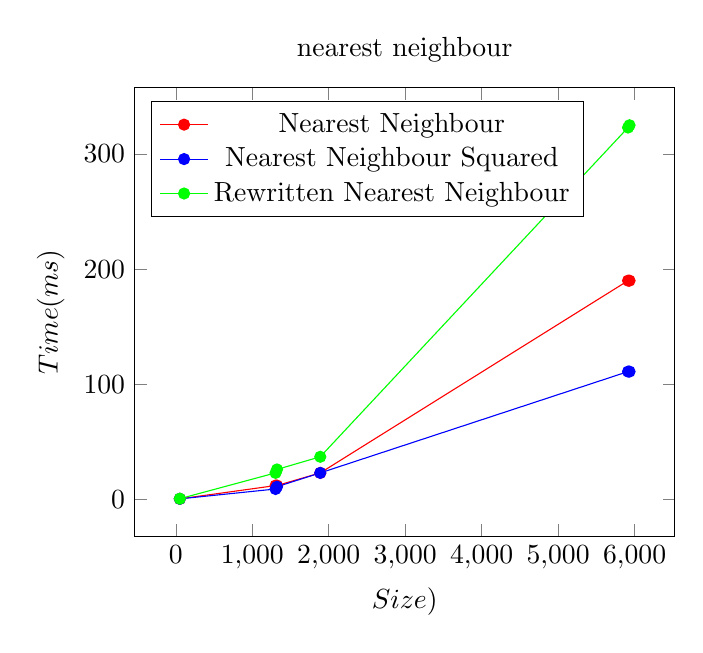
\begin{tikzpicture}
\begin{axis}[ 
title = nearest neighbour,
xlabel=$Size)$,
ylabel={$Time (ms)$},
legend pos=north west
] 
\addplot [red,mark=*] coordinates {(52,0.45) (1304,12) (1323,12) (1889,23) (5915,190) (5934,190)};
\addplot [blue,mark=*] coordinates {(52,0.45) (1304,9) (1323,11) (1889,23) (5915,111) (5934,111)};
\addplot [green,mark=*] coordinates {(52,0.59) (1304,23) (1323,26) (1889,37) (5915,323) (5934,325)};
\addlegendentry{Nearest Neighbour}
\addlegendentry{Nearest Neighbour Squared}
\addlegendentry{Rewritten Nearest Neighbour}
\end{axis}
\end{tikzpicture}

Out of the three basic nearest neighbour algorithms the fastest algorithm is the one that leaves the distances to be compared against in their squared form as well as storing the value from the function as a variable instead of computing it twice. From the graph it is clear that there is a gain in performance from 2000 points onwards. Once there are 5934 points the improved algorithm has a 41.57\% improvement on computation time of the algorithm. The reason for this improvement is due to the distance function which does the following calculation:

\begin{equation}
Distance = \sqrt{x^2 + y^2}
\end{equation}
Where $x$ is (point A.x - point B.x) and $y$ is (point A.y - point B.y).



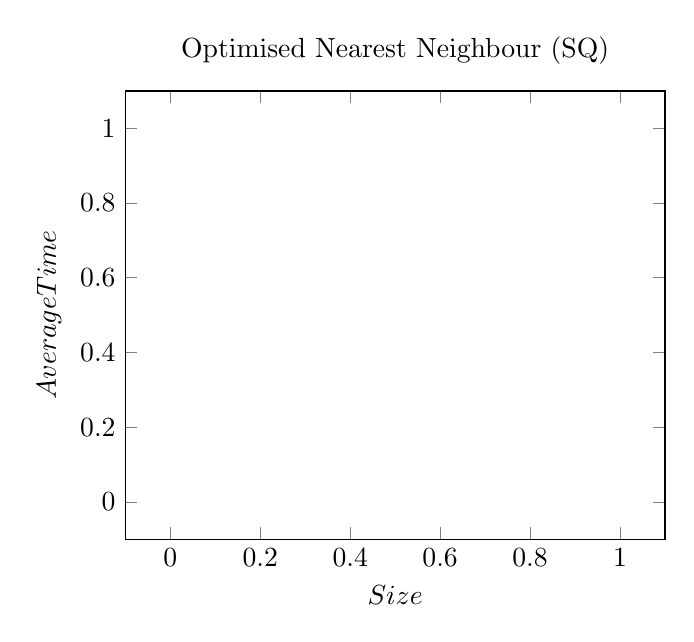
\begin{tikzpicture}
\begin{axis}[ 
title = Optimised Nearest Neighbour (SQ), 
xlabel=$Size$,
ylabel={$Average Time$}
] 
\end{axis}
\end{tikzpicture}

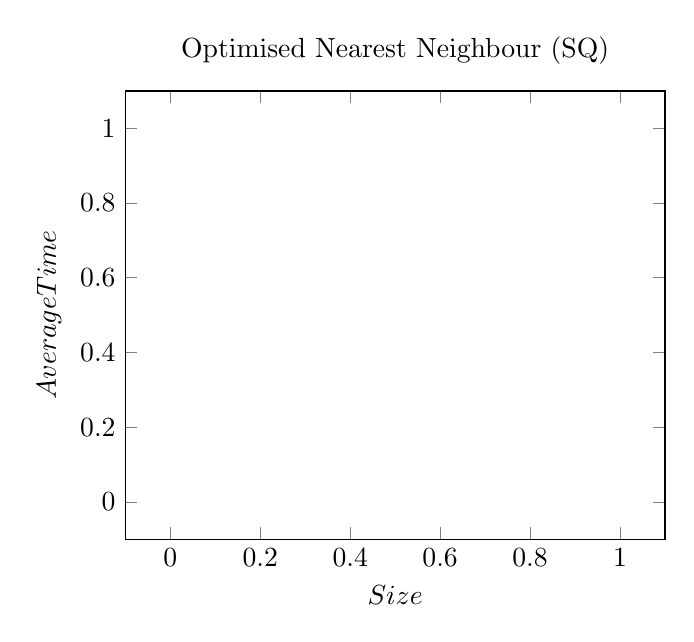
\begin{tikzpicture}
\begin{axis}[ 
title = Optimised Nearest Neighbour (SQ), 
xlabel=$Size$,
ylabel={$Average Time$}
] 
\end{axis}
\end{tikzpicture}

The next series of graphs are to show the data size against the total distance the route provides. As the optimised and rewritten algorithms were only aiming to improve the time taken to calculate the nearest neighbour they will be omitted as the route is the exact same as the nearest neighbour and evidence of this is provided in the tables above. 



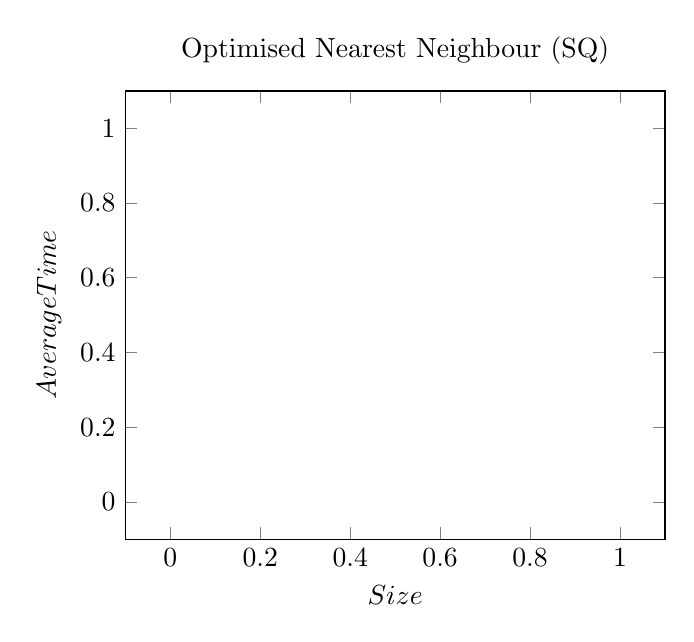
\begin{tikzpicture}
\begin{axis}[ 
title = Optimised Nearest Neighbour (SQ), 
xlabel=$Size$,
ylabel={$Average Time$}
] 
\end{axis}
\end{tikzpicture}
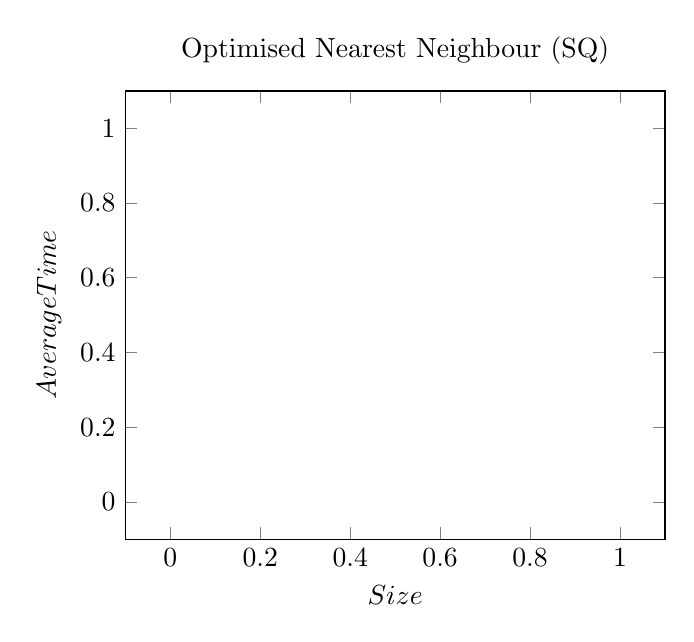
\begin{tikzpicture}
\begin{axis}[ 
title = Optimised Nearest Neighbour (SQ), 
xlabel=$Size$,
ylabel={$Average Time$}
] 
\end{axis}
\end{tikzpicture}
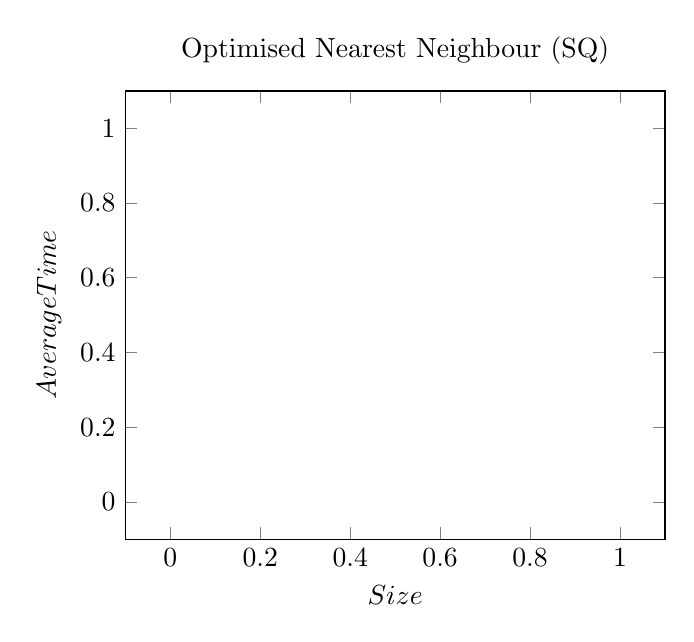
\begin{tikzpicture}
\begin{axis}[ 
title = Optimised Nearest Neighbour (SQ), 
xlabel=$Size$,
ylabel={$Average Time$}
] 
\end{axis}
\end{tikzpicture}
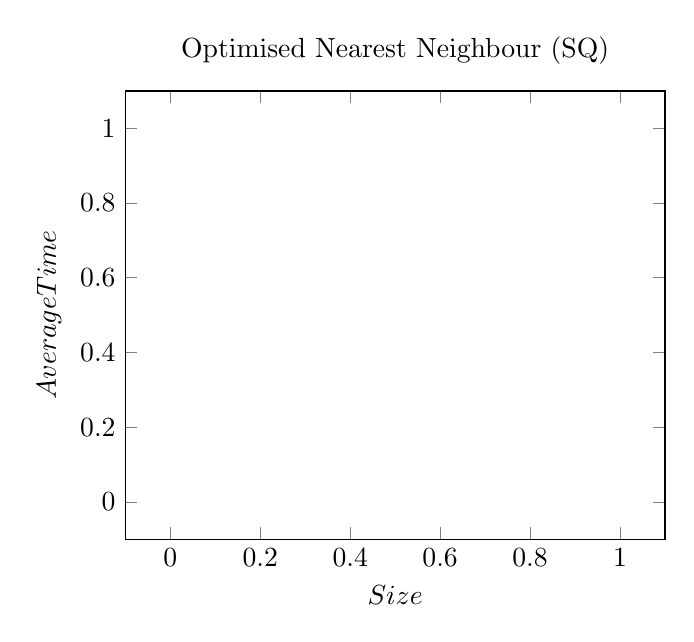
\begin{tikzpicture}
\begin{axis}[ 
title = Optimised Nearest Neighbour (SQ), 
xlabel=$Size$,
ylabel={$Average Time$}
] 
\end{axis}
\end{tikzpicture}



\paragraph{Routes}

This section is simply showing the output of each algorithm on some of the data sets. 

\underline{RL5915}

The route when it is unsorted looks like:

\begin{figure}
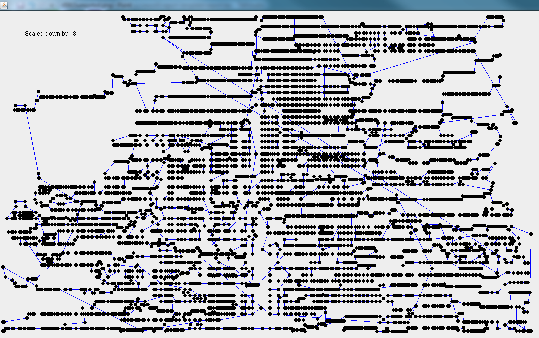
\includegraphics[width=\columnwidth]{images/rl5915nn.png}
\end{figure}
\section{Conclusion}

Due to the nature of the nearest neighbour algorithm some of the variations implemented would only result in a difference in time taken to compute the algorithm. However it is possible to compare the nearest neighbour with nearest x and nearest y as they produce different routes. 



To summarise what has been found from this investigation of the nearest neighbour algorithm in order to solve the travelling salesman problem. The algorithm provides a decent solution in a relatively quick time as long as there is a small 
% \section*{Acknowledgements}


\bibliographystyle{acmsiggraph}
\bibliography{report}

\end{document}

